\section{\gls{DPR} for External Fault Mitigation}\label{ExternalFaults}
Redundancy is a necessary feature to increase the dependability of a system.
Systems that have a need for high dependability encompass e.g. any safety critical system where a fault can result in the harm or even loss of human life.
Systems where maintenance may be difficult or expensive are another set of examples where redundancy is useful.
Redundancy can be achieved through the provision of multiple hardware entities that perform the same task.
If one hardware entity fails, another can take over and supply the expected functionality.
This can get expensive when there are multiple smaller hardware entities that perform specific computational work. 
To reduce space usage and cost, a general purpose \gls{CPU} can be used.
This \gls{CPU} can then emulate the functionality of the faulty hardware and thereby mitigates the fault. 
But this approach introduces new margin for error, as a two-pronged development may lead to discrepancies.
Another issue is real-time requirements that need to be fulfilled.
A regular \gls{CPU} may not be able to provide concurrent computations or the required performance, as the emulated hardware (or software) may be too complex.

A solution to these problems is the usage of \glspl{FPGA} as means of redundancy. 
As the \gls{FPGA} can be reconfigured with different functionality during runtime, it reduces the total amount of hardware that is needed to achieve redundancy.
Unlike \glspl{CPU}, \glspl{FPGA} provide better means for concurrent computation and are suitable to emulate multiple faulty hardware entities in a more appropriate manner. %TODO: Citation needed

Surprisingly, this approach is not very common in current literature, although the idea is explored by \cite{crdl2002} in the year 2002 in the context of \glspl{ECU} for the automotive industry.

The next section will describe the proposed concept by \cite{crdl2002} in more detail.

\subsection{\gls{DPR} for automotive applications}
A fail-safe circuit that is instantiated with \gls{DPR} is presented by \cite{crdl2002}. 
This circuit is meant to compensate the real-time functionality of a faulty \gls{ECU} and thereby provides redundancy.
This approach follows the goal of the reduction of hardware costs and the reduction of power and space needs, especially when it is extended to provide multiple backup circuits for different \glspl{ECU}.
One important assumption that is made is that a graceful degradation of performance and functionality is permitted to a certain extent, as long as it does not interfere with the minimal requirements of a safe functionality (e.g. reduction of vehicle speed due to limited processing power).
This is a notable distinction to a fault-tolerant design, which is usually able to mitigate a fault and is still able to fulfil most of its intended functionality.

To achieve redundancy, the \gls{FPGA} is connected to the same bus as the \glspl{ECU} that are monitored (see also Figure \ref{fig:externalFaultMitigation}).
For each \gls{ECU} a \gls{RP} in the \gls{FPGA} is reserved and hosts a watchdog that monitors the status of the \gls{ECU}.
Through this approach, each \gls{ECU} can be handled individually, and a higher resilience against a single point of failure in the monitoring logic is achieved, i.e. the malfunction of one watchdog does not affect the functionality of the others.
This is also done to save area on the \gls{FPGA} due to limited resources.
When the watchdog registers a fault (i.e. the absence of datagrams from the \gls{ECU}), the backup circuit is instantiated in the same \gls{RP} as the watchdog and overrides its functionality.
The faulty \gls{ECU} tries to shut down all of its communication on the bus and the instantiated backup circuit takes over.
The user of the \gls{ECU} should not notice that the data is provided by another entity now.

This concept was implemented and evaluated for the engine controller (fuel injection) and the transmission controller and was able to achieve the required real-time properties (with a reconfiguration time of 440$\mu$s) for minimal engine-performance.
The usage of area and memory on the \gls{FPGA} is analysed thoroughly as both are scarce.
This problem vanishes in the context of technological progress (from 2002 to 2019).
For example, the watchdog entities don't need to reside within the \gls{RP} anymore and may be condensed into one bigger health monitor in the static area of the \gls{FPGA} at the expense of area. 
Memory for the partial bitstreams is cheaper and easier available also, which aids the goal of redundancy for as many modules as possible. 
\begin{figure}
    \includegraphics[width=\columnwidth]{./graphics/externalFault.pdf}
    %\resizebox{\columnwidth}{!}{

\tikzset{every picture/.style={line width=0.75pt}} %set default line width to 0.75pt        

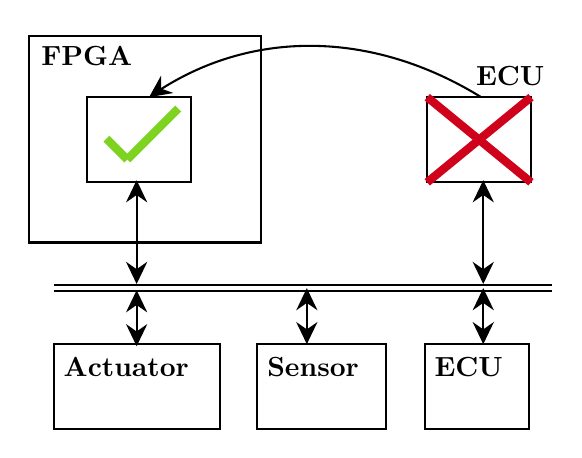
\begin{tikzpicture}[x=0.75pt,y=0.75pt,yscale=-1,xscale=1]
%uncomment if require: \path (0,279); %set diagram left start at 0, and has height of 279

%Shape: Rectangle [id:dp5787797491333819] 
\draw   (8,20.5) -- (120,20.5) -- (120,120) -- (8,120) -- cycle ;
%Shape: Rectangle [id:dp17505095690594463] 
\draw   (36,50) -- (86,50) -- (86,91) -- (36,91) -- cycle ;
%Shape: Rectangle [id:dp004684645465554249] 
\draw   (20,169) -- (100,169) -- (100,210) -- (20,210) -- cycle ;
%Shape: Rectangle [id:dp2725857150503048] 
\draw   (118,169) -- (180,169) -- (180,210) -- (118,210) -- cycle ;
%Shape: Rectangle [id:dp2885393682660524] 
\draw   (200,50) -- (250,50) -- (250,91) -- (200,91) -- cycle ;
%Shape: Rectangle [id:dp4969175268738504] 
\draw   (199,169) -- (249,169) -- (249,210) -- (199,210) -- cycle ;
%Straight Lines [id:da8580754234796655] 
\draw [color={rgb, 255:red, 208; green, 2; blue, 27 }  ,draw opacity=1 ][line width=3]    (200,50) -- (250,91) ;


%Straight Lines [id:da5772916268060835] 
\draw [color={rgb, 255:red, 208; green, 2; blue, 27 }  ,draw opacity=1 ][line width=3]    (250,50) -- (200,91) ;


%Curve Lines [id:da5702734861080319] 
\draw    (68.1,48.54) .. controls (114.3,17.01) and (173.3,17.5) .. (226,50) ;

\draw [shift={(66,50)}, rotate = 324.64] [fill={rgb, 255:red, 0; green, 0; blue, 0 }  ][line width=0.75]  [draw opacity=0] (10.72,-5.15) -- (0,0) -- (10.72,5.15) -- (7.12,0) -- cycle    ;
%Straight Lines [id:da7282259837027933] 
\draw [color={rgb, 255:red, 126; green, 211; blue, 33 }  ,draw opacity=1 ][line width=3]    (80,55.5) -- (55.5,80) ;


%Straight Lines [id:da7142424530641487] 
\draw [color={rgb, 255:red, 126; green, 211; blue, 33 }  ,draw opacity=1 ][line width=3]    (55.5,80) -- (45.5,70) ;


%Straight Lines [id:da36465994520752654] 
\draw    (20,140.5) -- (260,140.5)(20,143.5) -- (260,143.5) ;


%Straight Lines [id:da9447465253235761] 
\draw    (227,92) -- (227,138) ;
\draw [shift={(227,140)}, rotate = 270] [fill={rgb, 255:red, 0; green, 0; blue, 0 }  ][line width=0.75]  [draw opacity=0] (10.72,-5.15) -- (0,0) -- (10.72,5.15) -- (7.12,0) -- cycle    ;
\draw [shift={(227,90)}, rotate = 90] [fill={rgb, 255:red, 0; green, 0; blue, 0 }  ][line width=0.75]  [draw opacity=0] (10.72,-5.15) -- (0,0) -- (10.72,5.15) -- (7.12,0) -- cycle    ;
%Straight Lines [id:da358175601755349] 
\draw    (60,92) -- (60,138) ;
\draw [shift={(60,140)}, rotate = 270] [fill={rgb, 255:red, 0; green, 0; blue, 0 }  ][line width=0.75]  [draw opacity=0] (10.72,-5.15) -- (0,0) -- (10.72,5.15) -- (7.12,0) -- cycle    ;
\draw [shift={(60,90)}, rotate = 90] [fill={rgb, 255:red, 0; green, 0; blue, 0 }  ][line width=0.75]  [draw opacity=0] (10.72,-5.15) -- (0,0) -- (10.72,5.15) -- (7.12,0) -- cycle    ;
%Straight Lines [id:da07393951188629155] 
\draw    (60,145) -- (60,168) ;
\draw [shift={(60,170)}, rotate = 270] [fill={rgb, 255:red, 0; green, 0; blue, 0 }  ][line width=0.75]  [draw opacity=0] (10.72,-5.15) -- (0,0) -- (10.72,5.15) -- (7.12,0) -- cycle    ;
\draw [shift={(60,143)}, rotate = 90] [fill={rgb, 255:red, 0; green, 0; blue, 0 }  ][line width=0.75]  [draw opacity=0] (10.72,-5.15) -- (0,0) -- (10.72,5.15) -- (7.12,0) -- cycle    ;
%Straight Lines [id:da8542656416019287] 
\draw    (142,144) -- (142,167) ;
\draw [shift={(142,169)}, rotate = 270] [fill={rgb, 255:red, 0; green, 0; blue, 0 }  ][line width=0.75]  [draw opacity=0] (10.72,-5.15) -- (0,0) -- (10.72,5.15) -- (7.12,0) -- cycle    ;
\draw [shift={(142,142)}, rotate = 90] [fill={rgb, 255:red, 0; green, 0; blue, 0 }  ][line width=0.75]  [draw opacity=0] (10.72,-5.15) -- (0,0) -- (10.72,5.15) -- (7.12,0) -- cycle    ;
%Straight Lines [id:da22998818326497883] 
\draw    (227,144) -- (227,167) ;
\draw [shift={(227,169)}, rotate = 270] [fill={rgb, 255:red, 0; green, 0; blue, 0 }  ][line width=0.75]  [draw opacity=0] (10.72,-5.15) -- (0,0) -- (10.72,5.15) -- (7.12,0) -- cycle    ;
\draw [shift={(227,142)}, rotate = 90] [fill={rgb, 255:red, 0; green, 0; blue, 0 }  ][line width=0.75]  [draw opacity=0] (10.72,-5.15) -- (0,0) -- (10.72,5.15) -- (7.12,0) -- cycle    ;

% Text Node
\draw (36,30) node  [align=left] {\textbf{FPGA}};
% Text Node
\draw (240,40) node  [align=left] {\textbf{ECU}};
% Text Node
\draw (220,180) node  [align=left] {\textbf{ECU}};
% Text Node
\draw (145,180) node  [align=left] {\textbf{Sensor}};
% Text Node
\draw (55,180) node  [align=left] {\textbf{Actuator}};


\end{tikzpicture}
}
    \caption{External Fault Mitigation - functionality from a faulty \gls{ECU} is provided by a module (instantiated with \gls{DPR}) within the \gls{FPGA}}\label{fig:externalFaultMitigation}
\end{figure}
\subsection{Possible obstacles}
The work of \cite{shanker2016} identifies some obstacles that prevent \gls{DPR} in combination with \glspl{FPGA} for redundancy from a wider adaption through the industry and research.  

\begin{itemize}
\item \glspl{FPGA} are still expensive in comparison to \glspl{ECU}.
\item Significant expertise and initial development effort is needed.
\item Validation and certification concerns due to the difference to normal software architectures.
\item \gls{DPR} requires low-level access to hardware, which is contradictory to the abstraction goals of \gls{AUTOSAR}.
\end{itemize}
